%----------------------------------------------------------------------------
\chapter{Megvalósítás}
%----------------------------------------------------------------------------

{\color{red} Először valami bla-bla}



%----------------------------------------------------------------------------
\section{Alapok}
%----------------------------------------------------------------------------



Az OpenCV remek keretrendszer, rengeteg gyakran használt algoritmust implementáltak benne, viszont felépítését tekintve procedurális. Jelen feladatom megoldása során törekedtem az átlátható és jól struktúrált kód kialakítására, így ahol szükségesnek éreztem osztályokba szerveztem a logikát.

OpenCV-ben a legtöbb adatot egy mátrix (\texttt{cv::Mat}) adattípus reprezentál, ide értve a matematikai értelemben vett mátrixokat és a képeket is. Egy ilyen mátrix lényegében egy kétdimenziós tömb, melynek elemei lehetnek skalárok, de több-dimenziós vektorok is (több csatornás).

Elsőnek a \texttt{Camera} osztály, és annak konkrét implementáció készültek el, elfedve azt, hogy éppen a valódi kamerából kérünk le képkockákat, vagy fájlból olvassuk ki azokat. Ebből adódóan a \texttt{RealCamera} lényegében becsomagolja az OpenCV-s \texttt{VideoCapture} osztályt, és a \texttt{Camera} absztakt osztály közös interfészt nyújt a fájlból történő olvasáshoz is a \texttt{FakeCamera} számára. Ez főleg a tesztelés során volt hasznos, hogy egy adott jelenetet elég volt egyszer felvenni, és utána azt tudtam bemenetként használni. Az osztálydiagram \aref{fig:cd:camera}. ábrán látható.

A \texttt{cameraMatrix} attribútum jelöli a \textit{kamera-mátrix}ot és a \texttt{distCoeffs} attribútum a torzítási együtthatókat (lásd \aref{sec:pinhole}. szekció). Mivel ezek egy kamerára nézve időben állandóak, ezért csak egyszer kell őket meghatározni. A \texttt{readCalibration()} metódus szolgál ezek külső fájlból történő beolvasásukra. Miután rendelkezésre állnak ezek a paraméterek, akkor a \texttt{readUndistorted()} metódus segítségével olvashatok be rektifikált képet. A másik 3 metódus megfelel az azonos nevű metódusoknak a \texttt{cv::VideoCapture} osztályban \cite{cv_video}, ahol a \texttt{grab()} egy képkockát szerez az eszköztől, de nem olvassa (dekódolja) ki, míg a \texttt{retrieve()} ezt teszi. Ezt a kombinációt több kamerás rendszernél célszerű használni, úgy, hogy először mindegyik kamerán meghívjuk a \texttt{grab()}-et, majd utána lekérjük a képeket (amely művelet időigényes). Ezzel a módszerrel érhető el, hogy időben a lehető legközelebb legyenek a különböző kamerákból lekért képkockák egymáshoz. A \texttt{read()} a kettőt kombinálja kényelmi szempontból.

\begin{figure}[tbh]
\centering

\begin{tikzpicture} 

\begin{abstractclass}[text width=7 cm]{Camera}{0, 0}
\attribute   {+ cameraMatrix : Mat}
\attribute   {+ distCoeffs : Mat}

\operation   {+ readCalibration(fileName) : void}
\operation   {+ readUndistorted(outputImg) : void}
\operation[0]{+ grab() : void}
\operation[0]{+ retrieve(outputImg) : void}
\operation[0]{+ read(outputImg) : void}
\end{abstractclass}

\begin{class}[text width=5 cm]{RealCamera}{-4, -5.5}
\inherit{Camera}
\operation{+ grab() : void}
\operation{+ retrieve(outputImg) : void}
\operation{+ read(outputImg) : void}
\end{class}

\begin{class}[text width=5 cm]{DummyCamera}{4, -5.5}
\inherit{Camera}
\operation{+ grab() : void}
\operation{+ retrieve(outputImg) : void}
\operation{+ read(outputImg) : void}
\end{class}

\end{tikzpicture}

\caption{Osztályok a kamerához kezeléséhez \label{fig:cd:camera}}
\end{figure}


\section{Kalibráció}

Elsőként meg kell határoznom a kamerák már előbb is említett belső paramétereit. A módszert \aref{sec:pinhole}. szekcióban mutattam be, a következőkben ennek megvalósítását tárgyalom. Ehhez készült egy segédosztály \texttt{Calibration} néven, melynek feladata, hogy kellő információ után meghatározza a kamera-mátrixot és a torzítási együtthatókat és kiírja ezeket egy fájlba, hogy azt vissza tudjuk olvasni.

\begin{figure}[tbh]
\centering

\begin{tikzpicture} 

\begin{class}[text width=7 cm]{Calibration}{0, 0}
\attribute{- camera : Ptr<Camera>}
\attribute{- corners : vector<vector<Point2f>{}>}
\attribute{- cameraMatrix : Mat}
\attribute{- distCoeffs : Mat}

\operation{+ Calibration(camera)}
\operation{+ acquireFrame() : bool}
\operation{+ calibrate() : void}
\operation{+ save(fileName) : void}
\end{class}

\end{tikzpicture}

\caption{\texttt{Calibration} osztály \label{fig:cd:calibration}}
\end{figure}

Konstruktorban át kell neki adni a kamerára vonatkozó pointert, amitől a képeket kell majd lekérnie. Az \texttt{acquireFrame()} metódus szerepe, hogy a kamera aktuális képkockáját megszerezze, megkeresse a képen a sakktáblát, és a sakktábla sarokponjaihoz tartozó koordinátákat a \texttt{corners} listához fűzze. Visszatérési értékben jelzi, hogy az adott képen sikeres volt-e a detekció. Belsőleg a \texttt{cv::findChessboardCorners()} OpenCV-s függvényt hívja, amelynek átadva egy fekete-fehér képet, megkapható a képen látható sakktábla sarokpontjainak képpontjai. Kellő képkocka után a \texttt{calibrate()} metódus segítségével a kérdéses két mátrix (\texttt{cameraMatrix}, \texttt{distCoeffs}) kiszámolható. Itt a \texttt{cv::calibrateCamera()} függvényt hívom segítségül, melynek két fontos bemeneti paraméterét emelem ki: az sarokpontok valóvilágbeli koordinátái, és a képeken detektált képpontjai sorfolytonosan (\texttt{corners}). A valóvilágbeli $(x, y, z)$ koordinátákat az egyszerűség kedvéért úgy választottam, hogy $z \equiv 0$, és $x$ valamint $y$ egész számok úgy, hogy a sakktábla bal felső sarka $(0, 0, 0)$, jobb alsó sarka pedig -- $9\times 6$-os sakktáblát használva -- $(9, 6, 0)$. A \texttt{save()} pedig kimenti a paramétereket olyan formátumban, amiből a \texttt{Camera::readCalibration()} vissza tudja olvasni.


\subsection{Kamerák pozíciójának meghatározása világkoordinátákban}


Rögzített kamerák révén lehetőségem adódik, hogy előre meghatározzam a kamerák pozícióját és nézőpontjuk irányát. Erre egy kalibrációs objektumot használok, szintén egy sakktáblát. Amennyiben megadom a sakktábla sarokpontjainak koordinátáit az előbbiekkel egyező módon, akkor a sakktábla rögzítésével a térben, a koordinátarendszert is rögzítem. 

Az OpenCV-ben erre a célra van a \texttt{solvePnP} függvény, mely 3D-2D pont-összerendelésekből, kiszámolja a forgatási és eltolási vektort, amik együttesen megadják a transzformációt a model-koordinátarendszerből a kamera koordinátarendszerébe. Ezen funkciót a \texttt{CameraPoseCalculator} osztály ágyazza be, és a két vektort pedig a \texttt{CameraPose} csomagolja össze egy perzisztálható osztályba, lásd \aref{fig:cd:pose}. ábra.

\begin{figure}[tbh]
\centering

\begin{tikzpicture} 

\begin{class}[text width=5.3 cm]{CameraPoseCalculator}{-8.5, -0.50}
\attribute{- cam : Ptr<Camera>}

\operation{+ CameraPoseCalculator(cam)}
\operation{+ calculator() : bool}
\end{class}

\begin{class}[text width=5 cm]{CameraPose}{0, 0}
\attribute{+ rvec : Mat}
\attribute{+ tvec : Mat}

\operation{+ save(fileName) : void}
\operation{+ load(fileName) : void}
\operation{+ getRT() : Matx34d}
\end{class}

\aggregation{CameraPoseCalculator}{cameraPose~~~~~~~~~~}{1}{CameraPose}

\end{tikzpicture}

\caption{\texttt{CameraPoseCalculator} és \texttt{CameraPose} osztály \label{fig:cd:pose}}
\end{figure}

A \texttt{CameraPoseCalculator} osztály megkapja konstruktor argumentumaként annak a kamerára mutató pointerét, amelynek a külső paramétereit (forgatási és eltolási vektor, lásd \ref{sec:pinhole}. szekció vége) ki kell számolnia. A konkrét művelet végrehajtásáért a \texttt{calculator()} metódus felelős, amely a kamerától lekér egy képkockát, megkeresi rajta a sakktáblát, majd meghívja a \texttt{cv::solvePnP()} függvényt. Visszatérési értékben jelzi, hogy sikeres volt-e a detekció, ha igen, akkor lekérhető tőle a \texttt{CameraPose} példány. Ez utóbbi a \texttt{save()} és \texttt{load()} metódusokkal elmenthető és visszatölthető, így ameddig a kamerát nem mozgatjuk el, ez újra felhasználható. A \texttt{getRT()} metódus a forgatási vektorból forgatási mátrixot csinál (Rodrigues-féle forgatási formula \cite{camera-calib-3d}) és összefűzi azt az eltolási vektorral egy $3\times 4$-es $\Big(\,\mathbf{R}\,|\,\mathbf{t}\,\Big)$ forgatás-eltolás mátrixba.

A kamera külső paramétereinek meghatározása után már minden információ adott, hogy 3D-s pontok 2D-s vetületeit meg tudjam határozni a \texttt{cv::projectPoints()} függvény felhasználásával. \Aref{fig:pose}. ábrán látható, hogy egy a sakktábla síkjába rajzolt négyzetrács, melynek egyik jelölt pontja a világ-koordinátarendszer origója.

\begin{figure}[tbh]
\centering
\begin{subfigure}[b]{.49\linewidth}
	\centering
	\includegraphics[width=205pt]{figures/pose0_180.png}
	\caption{Bal oldali kamera}
  \end{subfigure}
\begin{subfigure}[b]{.49\linewidth}
	\centering
	\includegraphics[width=205pt]{figures/pose1_180.png}
	\caption{Jobb oldali kamera}
  \end{subfigure}
\caption{Világ-koordinátarendszer jelölése a képeken \label{fig:pose}}
\end{figure}

%----------------------------------------------------------------------------
\section{Objektum detekció}
%----------------------------------------------------------------------------

A következőkben az objekumok detekciójáról lesz szó. Először bemutatok két megközelítést az előtér maszk meghatározásához, ami lényegében a két képen kijelöli a mozgó részek maszkját. Ezt követően a maszkokat szegmentálni kell különálló \textit{blob}okra, és ezeket a két képen egymásnak megfeleltetni, hogy megkapjuk egy objektum két maszkját.

    %----------------------------------------------------------------------------
    \subsection{Előtér maszk meghatározása}
    %----------------------------------------------------------------------------


\subsubsection{Előtér-háttér szegmentáció}

\Aref{sec:obj_detection}. szekcióban leírtam a mozgó objektumok detekciójának egy lehetséges megközelítését. A lényege, hogy egy háttér modellt építünk, és így mindig aktuálisan lekérhető az előtérhez tartozó maszk, ami kijelöli a mozgó objektumokat. A probléma megoldása két fázisra bontható: először egyetlen objektumot keresek és detektálok, majd később több mozgó objektumot is.

Mindkét fázisnak közös része a már említett modellépítés, melyhez az OpenCV-ben megtalálható \texttt{BackgroundSubtractorMOG2} osztályt \cite{opencv-mog} hívom segítségül. Példányosítás után a modell építése, és az aktuális maszk kinyerése az \texttt{apply} metódussal történik. \Aref{fig:my_mog2}. ábrán látható a kinyerhető maszkra egy példa.

\begin{figure}[tbh]
\centering
\begin{subfigure}[b]{.32\linewidth}
	\centering
	\includegraphics[width=137pt]{figures/image230.png}
	\caption{Statikus kép -- ,,háttér''}
  \end{subfigure}
\begin{subfigure}[b]{.32\linewidth}
	\centering
	\includegraphics[width=137pt]{figures/image343.png}
	\caption{Mozgó képsor egy képe}
  \end{subfigure}
\begin{subfigure}[b]{.32\linewidth}
	\centering
	\includegraphics[width=137pt]{figures/mask343.png}
	\caption{Kapott előtér maszk}
  \end{subfigure}
\caption{Példa az előtér maszkra \label{fig:my_mog2}}
\end{figure}

Megfigyelhető, hogy a maszk nem pusztán bináris, hanem azt is jelzi, amit az algoritmus árnyéknak gondol. A zajt a maszkon az erózió-dilatáció morfológiai módszerek segítségével tudjuk csökkenteni. Előbbi a kisméretű zajokat tünteti el, utóbbi pedig a lyukakat szünteti meg. OpenCV-ben ezek implementációi a \texttt{dilate} és \texttt{erode} függvények. Előbbi az adott pixelt a környezetében (amit egy kernel ír le) lévő maximális, míg utóbbi a minimális értékkel helyettesít. Én egy erózió-dilatáció-erózió lépéssorozatot használok: először az apróbb szemcsék szűnnek meg, utána a lyukak. Az utolsó erózió szerepe, hogy az objektumok szélén a dilatáció miatt jelentkező növekedést megszűntesse. Ennek eredménye látható \aref{fig:erosion_dilation}. ábrán.

\begin{figure}[tbh]
\centering
\begin{subfigure}[b]{.49\linewidth}
	\centering
	\includegraphics[width=205pt]{figures/mask343.png}
	\caption{Eredeti}
  \end{subfigure}
\begin{subfigure}[b]{.49\linewidth}
	\centering
	\includegraphics[width=205pt]{figures/mask343_fixed.png}
	\caption{Árnyékok kivétele és zajcsökkentés után}
  \end{subfigure}
\caption{Előtér maszk zajmentesítése \label{fig:erosion_dilation}}
\end{figure}

Megfigyelhető, hogy a bal oldali dobozhoz tartozó maszk része annyira zajos volt, hogy a nagy lyuk nem szűnt meg, míg a kevésbé zajos jobb oldali doboz rendben megmaradt. A maszkot alkalmazva az eredeti képre \aref{fig:mask_applied}. ábrán látható, hogy egy bizonyos hibahatáron belül sikeresnek tekinthető a mozgó részlet kijelölése.

\begin{figure}[tbh]
\centering
\begin{subfigure}[b]{.49\linewidth}
	\centering
	\includegraphics[width=205pt]{figures/image343.png}
	\caption{Eredeti kép}
  \end{subfigure}
\begin{subfigure}[b]{.49\linewidth}
	\centering
	\includegraphics[width=205pt]{figures/mask343_applied.png}
	\caption{A detektált előtér}
  \end{subfigure}
\caption{Előtér maszk alkalmazás az eredeti képre \label{fig:mask_applied}}
\end{figure}

    %----------------------------------------------------------------------------
    \subsubsection{Előtér meghatározása optikai folyamokkal \label{sec:of-mask}}
    %----------------------------------------------------------------------------
    
Másik megközelítésem, hogy már az előtér meghatározásához is az optikai folyamokat hívom segítségül. 

\Aref{chapter2}. fejezetben bemutattam a sűrű optikai folyamok meghatározására Gunner Farnebäck módszerét. OpenCV-ben ezt a \texttt{cv::calcOpticalFlowFarneback()} \cite{opencv-mog} függvény valósítja meg. Az algoritmus szempontjából fontos paraméterei közül kiemelnék párat:

\begin{enumerate}
\item \texttt{pyr\_scale} -- a már említett piramis-módszerhez kapcsolódó paraméter: azt definiálja, hogy rétegenként a következő réteg hányszorosa az előzőnek (ennek segítségével a nagy elmozdulások kisebbek lesznek a kisebb rétegeken)
\item \texttt{levels} -- piramis rétegeinek a száma, 1-nél csak az eredeti képet használja, továbbiak nélkül
\item \texttt{winsize} -- az ablak méret, amit a mintavételezéshez használ
\item \texttt{iterations} -- iterációk száma minden piramis rétegen
\end{enumerate}

Tekintve, hogy nekünk csak az a fontos, hogy a lehető leggyorsabban kapjunk elmozdulásvektorokat, a paramétereket a következőknek megfelelően állítottam be: ne építsünk piramist (\texttt{levels = 1}, így \texttt{pyr\_scale} beállítása lényegtelen), valamint kicsit ablakmérettel dolgozzunk ($3\times 3$, tehát \texttt{winsize = 3}), valamint rétegenként elég 1 iteráció (\texttt{iterations = 1}).

A kiszámolt vektormezőből pedig a maszkot úgy határozom meg, hogy minden, egységnél hosszabb (tehát legalább 1 pixelnyi a becsült mozgása) vektor végpontját megjelölöm. Ezáltal lényegében azon részeket határoztam meg, ahova éppen a pontok mozdultak, ez pedig pontosan azon részei a képnek, ahol az adott képkockán az előtérben mozgó objektumokat éppen várjuk. Az előzőekhez hasonlóan a maszkon itt is végzünk apró utófeldolgozást a dilatáció és erózió morfológiai műveletek segítségével. Az eredményt \aref{fig:of_mask}. ábra mutatja be. Megfigyelhető, hogy a jól textúrázott objektumokhoz nagyon jó maszkot kapunk, a textúrázatlan területeken pedig a pontokat úgy tekinti mintha statikusak lennének.

\begin{figure}[tbh]
\centering
\begin{subfigure}[b]{.32\linewidth}
	\centering
	\includegraphics[width=137pt]{figures/frame_ofmask_101.png}
	\caption{2. képkocka}
  \end{subfigure}
\begin{subfigure}[b]{.32\linewidth}
	\centering
	\includegraphics[width=137pt]{figures/frame_ofmask_104.png}
	\caption{3. képkocka}
  \end{subfigure}
\begin{subfigure}[b]{.32\linewidth}
	\centering
	\includegraphics[width=137pt]{figures/frame_ofmask_107.png}
	\caption{4. képkocka}
  \end{subfigure}\\
\begin{subfigure}[b]{.32\linewidth}
	\centering
	\includegraphics[width=137pt]{figures/mask_ofmask_101.png}
	\caption{2. maszk}
  \end{subfigure}
\begin{subfigure}[b]{.32\linewidth}
	\centering
	\includegraphics[width=137pt]{figures/mask_ofmask_104.png}
	\caption{3. maszk}
  \end{subfigure}
\begin{subfigure}[b]{.32\linewidth}
	\centering
	\includegraphics[width=137pt]{figures/mask_ofmask_107.png}
	\caption{4. maszk}
  \end{subfigure}
\caption{Egy jelenet 3 képkockája és ezekből az optikai folyamok felhaszánlásával kapott maszkok (már zajcsökkentés után) \label{fig:of_mask}}
\end{figure}


Az osztálydiagramot \aref{fig:cd:fg-mask-calc}. ábra mutatja be. \texttt{ForegroundMaskCalculator} osztály lényegében egy közös interfészt nyújt csak, valamint egy \texttt{morph()} metódust tartalmaz, mely a morfológiai műveleteket végzi el a maszkon. A \texttt{MOG2ForegroundMaskCalculator} az OpenCV-s \texttt{BackgroundSubtractorMOG2} osztály egy példányát csomagolja be, ami minden új képkockát megkap, és visszaadja a maszkot, az algoritmus által árnyéknak jelölt részeket a \texttt{removeShadows()} távolítja el. \texttt{OFForegroundMaskCalculator} pedig eltárolja az előző képkockát, és ebből meg az éppen aktuális képkockából \texttt{calcOpticalFlowFarneback()} segítségével a lehető leggyorsabban meghatározza a képkockákra az optikai folyamot, melyből aztán az előbbiekben ismertetett módszerrel a \texttt{getMaskFromFlow()} adja vissza a maszkot.

\begin{figure}[tbh]
\centering

\begin{tikzpicture} 

\begin{abstractclass}[text width=5.3 cm]{ForegroundMaskCalculator}{0, 0}

\operation   {\# morph(mask) : void}
\operation[0]{+ calculate(nextFrame) : Mat}

\end{abstractclass}

\begin{class}[text width=6.3 cm]{MOG2ForegroundMaskCalculator}{-3.8, -3.5}
\inherit{ForegroundMaskCalculator}
\attribute{- sub : BackgroundSubtractorMOG2}
\operation{- removeShadows(mask): void}

\operation{+ calculate(nextFrame) : Mat}
\end{class}

\begin{class}[text width=6.3 cm]{OFForegroundMaskCalculator}{3.8, -3.5}
\inherit{ForegroundMaskCalculator}
\attribute{- prevFrame : Mat}
\operation{- getMaskFromFlow(flow) : Mat}

\operation{+ calculate(nextFrame) : Mat}
\end{class}

\end{tikzpicture}

\caption{Előtér maszk meghatározására szolgáló implementációk \label{fig:cd:fg-mask-calc}}
\end{figure}

%----------------------------------------------------------------------------
\subsection{Egyetlen objektum detekciója}
%----------------------------------------------------------------------------

Kezdetben azzal az egyszerűsítéssel élek, hogy a képen csak egyetlen mozgó objektumot detektálok, mégpedig azt, amelyik a legnagyobb részt foglalja el a képeken. Ez nagyban egyszerűsíti a dolgokat, mert ahogy majd látni fogjuk a következő szekcióban, az optikai folyam meghatározására szükség lesz a képeken látható \textit{blob}ok (egy objektumhoz tartozó egybefüggő rész a képen) párosításra a kamerák képein. Mivel összesen egy blobot jelölök ki a képeken, ezek párosítása triviális, és nagy valószínűséggel ugyanazon objektumhoz tartoznak majd.

Ehhez először szükség van az összefüggő komponensek kiválasztására. Két módszer kínálkozik erre OpenCV-ben; az egyik a \texttt{findContours()} függvény, ami megkeresi a képen látható kontúrokat (paraméterezhető, hogy csak a legkülsőbbeket találja meg, a belső kontúrokat nem), a másik pedig a a \texttt{connectedComponentsWithStats()}, mely a 3.0-s verziótól érhető el. Az első abban különbözik az utóbbitól, hogy a kapott kontúrt felhasználva megkaphatjuk a belső területet (lyukak nélkül), míg utóbbi lényegében a maszk pixeleit címkézi fel, hogy melyik komponenshez tartoznak. Ezért én az előbbi használata mellett döntöttem. Miután megvannak ezek a kontúrok a belső területeket meghatározom a \texttt{cv::contourArea()} függvénnyel, és egy maximum kiválasztás után megkapom a legnagyobb területtel rendelkező komponens maszkjával. Mindkét képre elvégezve ezt, megkapom az egyik és másik képen a legnagyobb objektumhoz tartozó 1-1 maszkot. Az algoritmus eredmény \aref{fig:single-obj}. ábrán látható.

\begin{figure}[tbh]
\centering
\begin{subfigure}[b]{.49\linewidth}
	\centering
	\includegraphics[width=205pt]{figures/mask_ofmask_104.png}
	\caption{Eredeti maszk}
  \end{subfigure}
\begin{subfigure}[b]{.49\linewidth}
	\centering
	\includegraphics[width=205pt]{figures/mask_ofmask_104_selected.png}
	\caption{Detektált blobok, és fehérrel a legnagyobb}
  \end{subfigure}
\caption{Legnagyobb területű blob kijelölése \label{fig:single-obj}}
\end{figure}

%----------------------------------------------------------------------------
\subsection{Több objektum detekciója, párosítás a kamerák képein}
%----------------------------------------------------------------------------

A következő feladat, amit meg kell oldanom, az több objektum együttes detekciója, úgy, hogy a két képen az egymásnak megfelelő blobokat párosítsam. Ehhez jellegzetes pontokat, és ezekhez tartozó leírókat keresek, illetve számolok ki a képi információkból.

A szakirodalomban több algoritmust is találhatunk, mely vagy a jellegzetes pontok (\textit{feature}) detektálásában (pl. FAST \cite{FAST}, MSER \cite{MSER}), vagy ezen pontokhoz tartozó leírók (\textit{feature descriptor}) kinyerésében (pl. FREAK \cite{FREAK}), vagy mindkettőre használhatóak (pl. ORB \cite{ORB}, SIFT \cite{SIFT} és SURF \cite{SURF}). SIFT és a SURF a tradícionális leírók közé sorolhatóak abban a tekintetben, hogy vektor-alapú leírokat készítenek, ellenben az újabbakkal, amelyek bináris-füzéreket. Előbbi algoritmusok kiszámolása idő- és erőforrásigényes, valós idejű, valamint mobil eszközökön történő alkalmazásra kevésbéalkalmasak, ellenben utóbbiak igen, és a kinyert leírók összehasonlítása is gyors (Hamming-távolság). Dolgozatomnak nem célja ezek mélyreható vizsgálata és rangsorolása, de \cite{feature-detection-comparison} alapján először a FREAK-ket próbáltam meg alkalmazni több különböző forgatás- és skálainvariáns detektor által visszaadott kulcspontokra, sajnos kevés sikerrel. Minden bizonnyal a paraméterezést rontottam el, de nem sikerült javítanom a végeredményen. \cite{ORB} után az ORB-ot próbáltam ki, és már kielégítő eredményt kaptam, hasonlóan a SURF-fel végzett kísérletekhez, ellenben jóval kevesebb idő alatt, így ennél maradtam.

Miután mindkét képen megkerestem a jellegzetes pontokat, és kinyertem hozzájuk a leírókat, ezeket párosítanom kell. Ehhez használhatunk brute-force módszert (mindent mindennel összehasonlítva és kiválasztva a legközelebbit), vagy a FLANN (Fast Approximate Nearest Neighbor Search Library \cite{flann_pami_2014}) könyvtárat, melyhez OpenCV-ben is elkészült az interfész \cite{opencv-flann}. Ez első sorban arra használható, hogy gyorsan tudjunk több dimenziós vektortérben egy vektorhoz megkeresni a hozzá legközelebbi vektort, amely SIFT és SURF esetben ideális, de használható bináris leírókhoz is \cite{flann-binary}. Mivel a halmaz mérete, ahol a párosítást keressük, nem olyan nagy, hogy a brute-force módszer hátránya kiütközzön, ezért emellett maradtam, melynek OpenCV-ben az implementációját a \texttt{cv::BFMatcher} osztályban találjuk.

Végül a kapott párosításokat a fundamentális mátrix segítségével validálom és kiszűröm, vagyis megnézem, hogy a már használt epipoláris ($\mathbf{u}'^T \mathbf{F} \mathbf{u} = 0$) kényszer egy adott hibahatáron belül teljesül-e. Gondoljuk meg, hogy ettől még maradhat teljesen rossz párosítás is a halmazban, hiszen az adott ponthoz csak azt nézi meg, hogy a másik pont rajta van-e a hozzá tartozó epipoláris egyenesen. \Aref{fig:multi-obj-matches}. ábrán látható a legközelebbi 20 találat. 

\begin{figure}[tbh]
\centering

\begin{tikzpicture}[spy using outlines={circle,white,magnification=3,size=1.5cm, connect spies}]

\node {\includegraphics[width=400pt]{figures/multi_obj_matches.png}};
\spy on (-5.33,-1.5) in node [left] at (-5.5,0.5);
\spy on (2.0,-1.58) in node [left] at (4.7,-1.7);

\spy on (-1.8,-0.1) in node [left] at (-2.8,1.7);
\spy on (5.4,-0.14) in node [left] at (4,1.7);

%\tikzset{help lines/.style={color=blue!50}}
%\draw[thick,step=1cm,help lines] (-7,-2) grid (7,2);

\end{tikzpicture}

\caption{Blobok által kijelölt képrészleteken az egymásnak megfelelő pontok keresése. A találatok szempontjából érdemi rész látható, a 20 legközelebbi találattal és ezekből 1-1 kiemelve közelről \label{fig:multi-obj-matches}}
\end{figure}

Ezt követően a blobokat a következőképpen párosítom. Veszem azt a képet, amelyiken több blob van, mint a másikon (ha ugyanannyi, akkor a választás tetszőleges), majd egyesével az itt lévő blobokhoz megkeresem, hogy a benne lévő párosításbeli pontok párjainak többségét melyik másik képen lévő blob tartalmazza. Így kapok egy projekciót a több elemű halmazból a kisebbe. Nem feltétlen lesz minden blobnak párja (nem tartalmaz \textit{feature} pontot), valamint lehet, hogy több különböző blob is ugyanahhoz a blobhoz fog tartozni, ekkor ezeket eggyesítem. Így a végén a blobok egy részhalmazához egy kölcsönösen egyértelmű relációt, párosítást kapok, ezek jelölik ugyanazon objektum két maszkját a két képen. %\Aref{fig:multi-obj-matches} képrészleten látható objektumok esetén például a 367 talált párosításból a 1 objektumhoz tartozó maszkból atból összesen 30 volt két nem egymáshoz tartozó blobok között

Annak érdekében, hogy a következő lépéseket könnyebben tudjam tesztelni, aktívan fogom használni a csak egy objektum detekciójára képes algoritmust is, ezért a két megoldásnak interoperábilisnak kell lennie. Tehát mindkettő egy közös \texttt{ObjectSelector} absztrakt osztályból származik, lásd \ref{fig:cd:objectselector}. ábra. Későbbiekben fogjuk látni, hogy ennél a módszernél is jó, ha meghatározzuk az egymásnak megfelelő pontokat, így végülis mindkettő megkapja konstruktorában a \texttt{Matcher} osztály egy példányát, melyet a \texttt{ObjectSelector} őriz. A \texttt{Matcher} két képkockából és az előtér maszkokból meghatározza az egymásnak megfelelő pontokat ORB-bal, melyeket pontpáros listájaként ad vissza. Konstruktorában azért, hogy a találatokat szűrni tudja megkapja a kamera objektumokat és a fundamentális mátrixot. Mindkét konkrét \texttt{ObjectSelector} megvalósítás \texttt{Object} listával tér vissza, mely tartalmazza a két maszkot a két képen, valamint az összetartozó pontokat.


\begin{figure}[tbh]
\centering

\begin{tikzpicture} 

\begin{class}[text width=5.5 cm]{Matcher}{4.5, 0}

\operation{+ Matcher(cam1, cam2, F)}
\operation{+ match(imgs, masks) : ~~~~~~~ vector<pair<Point2f, Point2f>{}>}

\end{class}

\begin{abstractclass}[text width=7 cm]{ObjectSelector}{-3.8, 0}

\operation   {+ ObjectSelector(matcher)}
\operation[0]{+ select(frames, masks) : vector<Object>}

\end{abstractclass}


\aggregation{ObjectSelector}{matcher~~~~~~~~~~}{1}{Matcher}


\begin{class}[text width=7 cm]{SingleObjectSelector}{-3.8, -3}
\inherit{ObjectSelector}

\operation{+ SingleObjectSelector(matcher)}
\operation{+ select(frames, masks) : vector<Object>}
\end{class}

\begin{class}[text width=7 cm]{MultiObjectSelector}{4, -3}
\inherit{ObjectSelector}

\operation{+ MultiObjectSelector(matcher)}
\operation{+ select(frames, masks) : vector<Object>}
\end{class}

\begin{class}[text width=7.5 cm]{Object}{0, -6}
\operation{+ masks : vector<Mat>}
\operation{+ matches : vector<pair<Point2f, Point2f>{}>}
\end{class}

\draw[umlcd style dashed line,->] (SingleObjectSelector.south) ++
(-3,0) |- node [above,sloped,black,pos=0.75]{$ < <$ instantiate $ > >$} (Object);

\draw[umlcd style dashed line,->] (MultiObjectSelector.south) ++
(3,0) |- node [above,sloped,black,pos=0.75]{$ < <$ instantiate $ > >$} (Object);

\end{tikzpicture}

\caption{Objektumok kijelölését szolgáló osztályok \label{fig:cd:objectselector}}
\end{figure}



%----------------------------------------------------------------------------
\section{Optikai folyam meghatározása}
%----------------------------------------------------------------------------

\Aref{sec:of-mask}. szekcióban bemutattam, hogyan lehet felhasználni a sűrű optika folyamokat előtér maszk meghatározására, a következőkben pedig azt, hogyan lehet sűrű pontmegfeleltetést meghatározni segítségével a két kamera egy objektumhoz tartozó két képén.

Előzőekben bemutattam a \texttt{cv::calcOpticalFlowFarneback()} függvényt, és annak néhány paraméterét, amelyeket úgy állítottam be, hogy a lehető leggyorsabban kapjak még használható becslést a mozgásról. Most viszont fontos, hogy amit kapunk eredmény az pontosabb legyen, tehát ezeken kicsit változtatni kell. Ezért 6 szintes piramist (\texttt{levels = 6}), és köztük 0,75-ös skálázást (\texttt{pyr\_scale = 0.75}) állítottam be, hogy a nagyobb mozgásokat is detektálni tudjam. A gaussi zaj feltételezése miatt bekapcsoltam, hogy egyszerű dobozszűrő helyett gaussi filtert használjon az algoritmus, és az ehhez kapcsolódó paramétereket a dokumentációban adott javaslatok alapján állítottam be, valamint emiatt az ablakméretet is növeltem (\texttt{winsize = 21}). A futási idő természetesen függ a kép méretétől, így fontos, hogy kihasználjuk az objektum maszkjából nyerhető információt.

A következőkben \aref{fig:of_original}. ábrán látható két képkocka lesz a kiinduló állapot, már az előbbiekben bemutatott objektum detekció után, az előtér maszk által kijelölve. A képkockák két olyan kamera beállításal készültek, ahol a két kamera képsíkja nagyjából egybe esik (egy irányba néznek), és csak víszintes irányban vannak egymáshoz képest eltolva.

\begin{figure}[tbh]
\centering
\begin{subfigure}[b]{.49\linewidth}
	\centering
	\includegraphics[width=205pt]{figures/of_img_left_framed.png}
  \end{subfigure}
\begin{subfigure}[b]{.49\linewidth}
	\centering
	\includegraphics[width=205pt]{figures/of_img_right_framed.png}
  \end{subfigure}
\caption{Bal és jobb kamera által látott objektum kijelölve; a sárga keretek jelölik az objektumok befoglaló téglalapjait, a piros pedig ezen téglalapokat tartalmazó legkisebb területű téglalapot \label{fig:of_original}}
\end{figure}

Első megközelítésem, hogy a két objektum befoglaló téglalapját tekintem, és veszem azt a téglalapot, mely a legkisebb területű azok közül, amely mindkettőt tartalmazza. Kivágva ezt a téglalapot a két képből, két egyforma méretű képrészletet kapok, melyek külön-külön tartalmazzák a teljes objektumot. Ez látható \aref{fig:of_original}. ábrán pirossal jelölve. Erre a két részletre számolva optikai folyamot, 7 646 darab vektort kaptam, melyek közül néhányat vizualizáltam \aref{fig:bad0}. ábrán. A vektorok kezdő és végpontjaiból alkotok pontpárokat, ezeket tekintem egymásnak megfelelő pontoknak a két képen. Jól látható, hogy a kevés kirajzolt pontpárból egyik sem tekinthető jónak, mert a doboz különböző lapjaihoz tartozó pontok. Ez a nagy elmozdulás miatt van, hiába a piramis módszer, nem használható a végeredmény.

\begin{figure}[tbh]
\centering
\includegraphics[width=300pt]{figures/vis_bad_0.png}
\caption{Első megközelítés (36 958 vektor) \label{fig:bad0}}
\end{figure}

A következő lépésem, hogy meghatározom azt a vektort, amivel eltolva az egyik képet, az egymásnak megfelelő képpontok elmozdulásai a lehető legkisebbek lesznek. Ehhez először szükségem van néhány egymásnak megfelelő pontpárra.

Az objektumok meghatározásánál (legyen az egy vagy több), már meghatároztam néhány egymásnak megfelelő pontot, így ezeket itt fel tudom használni (\texttt{Object::matches}). Ezek után a párosítások jelentette vektorokból kell meghatároznom azt a vektort, amellyel az egyik képet eltolva az összetartozó pontok közötti távolság minimális. Azaz

\[\min_{\mathbf{v}(x, y)} \sum_{i=1}^{n} |\mathbf{v} - \mathbf{d_i}|\]

ahol $\mathbf{d_1}(x_1, y_1), \mathbf{d_2}(x_2, y_2), \ldots \mathbf{d_n}(x_n, y_n)$ a párosításban szereplő pontok közti távolságvektorok. Vagyis:

\[\min_{x, y} \sum_{i=1}^{n} \sqrt{(x-x_i)^2 + (y-y_i)^2}\]

{\color{red}Mivel a gyökvonás monoton, és a gyökvonás ezért a minimalizálásnál elhagyhatjuk. Így viszont ez megfogalmazható legkisebb négyzetek problémának, ami megoldható szinguláris érték szerinti felbontással.} \Aref{fig:shifted}. ábrán látható az eltolás előtt és után az objektum helyzete a két képen.

\begin{figure}[tbh]
\centering
\begin{subfigure}[b]{.49\linewidth}
	\centering
	\includegraphics[height=205pt]{figures/before_shift.png}
  \end{subfigure}
\begin{subfigure}[b]{.49\linewidth}
	\centering
	\includegraphics[height=205pt]{figures/after_shift.png}
  \end{subfigure}
\caption{Az objektum elhelyezkedése a kamerák képein (egymás alatt a két kamera képe) eredetileg és a kiszámolt vektorral való eltolás után. \label{fig:shifted}}
\end{figure}

Optikai folyamok számítása esetén két jelenséget nem szabad figyelmen kívül hagynunk: egyik a textúrázatlanság, a másik pedig a kitakart pontok problémája. Ezeken az optikai folyam rektifikációja segíthet. \cite{optical-flow-rectification}-ban You Yang és társai egy bináris függvényt javasolnak a textúrázatlanság eldöntésére:

\[
    \zeta(\Omega_\mathbf{X})= 
\begin{cases}
    0,              & \text{ha } \sigma(I_{\forall \mathbf{Y}\in\Omega_\mathbf{X}} - I_\mathbf{X}) < \varepsilon_\Omega\\
    1,              & \text{különben}
\end{cases}
\]

ahol $\Omega_\mathbf{X}$ jelöli $\mathbf{X}$ képpont egy környezetét, $I_\mathbf{X}$ az $\mathbf{X}$ pont intenzitását, $\sigma(.)$ a szórás-operátort egy halmazra nézve, valamint $\varepsilon_\Omega$ egy küszöbértéket, ami konstans. Úgy találták, hogy $\varepsilon_\Omega = 6$ választással jó eredményeket értek el, így én is ezt használtam. A mintaképek pontjaira kiszámolve ezt a függvényt, \aref{fig:textures}. ábrán látható maszkokat kaptam.

\begin{figure}[tbh]
\centering
\includegraphics[width=300pt]{figures/textures.png}
\caption{$\zeta$ függvény alkalmazva az objektum összes pontjára \label{fig:textures}}
\end{figure}

{\color{red}A kitakart pontok kiszűrésére én \cite{optical-flow-rectification}-től eltérő megközelítést alkalmaztam.} Legyen két képkocka $K_1$ és $K_2$, valamint $F_{1, 2} = \mathcal{F}(K_1, K_2)$ és $F_{2, 1} = \mathcal{F}(K_2, K_1)$, ahol $\mathcal{F}$ jelöli két képkocka közti optikai folyam operátort, melynek eredménye egy vektormező ($F_{1, 2}, F_{2, 1} : \mathbb{R}^2 \rightarrow \mathbb{R}^2$). Gondoljuk meg, hogy ha $x\in K_1$ és $x + F_{1,2}(x) = x' \in K_2$, akkor $x' + F_{1,2}(x') \approx x \in K_1$, vagyis ha egy $x$ pont $K_1$-ről $K_2$-re az $x'$ pontba mozog, akkor visszafelé nézve $x'$ pontnak ideális esetben $x$ pontba kell, hogy mozogjon. Tehát oda-vissza számolva 1-1 optikai folyamot a kitakart pontokat kiszűrhetjük, hiszen a másik irányban nem fogjuk megtalálni a párosítást.

A fent leírtakat az \texttt{OpticalFlowCalculator} osztályban implementáltam (rövid áttekintő látható \aref{fig:cd:ofcalc}. ábrán). Egy publikus metódusa van \texttt{calcDenseMatches()} néven, mely megkapja a két képkockát és egy objektumot, amelyre a sűrű pontmegfeleltetést szeretnénk számolni. Ez lényegében három dolgot csinál: meghatározza a textúrázott régiókat (\texttt{calcTexturedRegion}) a két képen, meghatározza oda és vissza az optikai folyamokat (\texttt{calcOpticalFlows}), majd ezek alapján meghatározza a párosításokat (\texttt{collectMatchingPoints}).

\begin{figure}[tbh]
\centering

\begin{tikzpicture} 

\begin{class}[text width=8 cm]{OpticalFlowCalculator}{0, 0}

\attribute{- frames : Mat[]}
\attribute{- masks : Mat[]}
\attribute{- texturedRegions : Mat[]}

\operation{- calcTexturedRegion(frame, mask) : Mat}
\operation{- calcOpticalFlows() : vector<Mat>}
\operation{- collectMatchingPoints(flows) : pair<vector<Point2f>, vector<Point2f>{}>}

\operation{+ calcDenseMatches(frames, object) : pair<vector<Point2f>, vector<Point2f>{}>}

\end{class}

\end{tikzpicture}

\caption{Sűrű pontmegfeleltetések optikai folyamok segítségével meghatározó \texttt{OpticalFlowCalculator} osztály \label{fig:cd:ofcalc}}
\end{figure}

Az algoritmust lefuttatva egész pontos párosításokat kaptam, \aref{fig:vis_full}. ábra mutat ezek közül néhányat. Összesen 16 841 pár jött létre, tehát ennyit fogok tudni felhasználni a háromszögeléshez. %Vessük össze ezt a SURF leírókka történő párosításnál nyert 100, majd abból meghagyott 25 párral, számottevő a különbség.

\begin{figure}[tbh]
\centering
\includegraphics[width=300pt]{figures/vis_full.png}
\caption{Végső párosítás az optikai folyamok segítségével (16 841 vektor) \label{fig:vis_full}}
\end{figure}

%----------------------------------------------------------------------------
\section{Háromszögelés}
%----------------------------------------------------------------------------

Ahogy \aref{sec:triangulation}. alfejezetben bemutattam az elméleti hátteret, a következőkben ennek implementálását mutatom be.

\subsection{OpenCV-s függvényekkel}

OpenCV \texttt{cv::triangulatePoints} függvényben a \textit{Linear-LS} (lineáris legkisebb négyzetek) módszer van implementálva. Az interneten rákeresve több fórumban is találtam arra vonatkozó információkat, hogy sokan küzködnek ennek meghívásával. A dokumentáció \cite{camera-calib-3d} alapján sztereó-kalibráció során nyert projekciós mátrixokat várja a pontpárok mellett paraméterül. Az én esetemben, a kamerák nincsenek sztereó-kalibrálva, de a két projekciós mátrix megvan. Ennek ellenére a kimeneti 3D-s koordináták használhatatlanok voltak. Kis kutatás után az \texttt{cv::undistortPoints()} függvény meghívása jelentette a megoldást. Ez először normalizálta őket, vagyis:

\[\left(\begin{array}{c} u' \\ v' \\ 1 \end{array}\right) = {\underbrace{\left(\begin{array}{ccc}
f_x & 0 & o_x \\ 
0 & f_y & o_y \\
0 & 0 & 1
\end{array}\right)}_{\hbox{kamera-mátrix}}}^{-1} \left(\begin{array}{c} u \\ v \\ 1 \end{array}\right)\]

ahol $(u', v')$ az $(u, v)$ pont normalizáltja (kamera-mátrixtól független koordináták), majd a torzítási együtthatóakat felhasználva az $(u', v')$ pontoknak meghatározta a javított koordinátájukat. Ezután a \texttt{cv::triangulatePoints} függvénynek a projekciós mátrixok helyett csak az $\Big(\,\mathbf{R}\,|\,\mathbf{t}\,\Big)$ mátrixokat kellett átadnom. Fontos, hogy az előbbiekben kialakított pontpárosítás azon osztályához tartozó pontokat, melyek az eltolt képhez tartoznak, az eltoláshoz használt vektor ellentettjével vissza kell tolni, hogy valós koordinátákat kapjunk.

Miután megvannak a valóvilágbeli koordináták ezek pontosságát a képsíkokra történő visszavetítéssel vizsgáltam meg. A pontokat a \texttt{cv::projectPoints} függvénnyel vetítettem a bal és jobb oldali kamera képére, majd a vetített és az eredeti pontok távolságainak átlagát -- átlagos visszavetítési hiba -- vizsgáltam. Ez az előzőekben mutatott bemenetre 8,68716 pixel lett, és \aref{fig:cv-triangulation}. ábrán látható az eredményeket bemutató két vizualizáció, melyeken a szín a pontok $z$ koordinátáját jelzi.

\begin{figure}[tbh]
\centering
\begin{subfigure}[b]{.49\linewidth}
	\centering
	\includegraphics[width=205pt]{figures/visu_left.png}
	\caption{Bal oldali kamera nézőpontjából nézve \label{fig:cv-triangulation-a}}
  \end{subfigure}
\begin{subfigure}[b]{.49\linewidth}
	\centering
	\includegraphics[width=205pt]{figures/visu_pcl.png}
	\caption{PCL vizualizációs szoftverrel ráközelítve}
  \end{subfigure}
\caption{Háromszögelés \textit{Linear-LS}-sel. Jól látható a közeli nézőpontból, hogy egy kissé hullámos lett a felület \label{fig:cv-triangulation}}
\end{figure}

Az OpenCV keretrendszerben megtalálhatjuk a \cite{hartley-triangulation}-ben leírt optimális, de polinomiális algoritmust is implementálva \texttt{cv::correctMatches()} néven, amely a fundamentális mátrix segítségével \aref{sec:triangulation}. szakaszban említett módon javítja a pontpárokat, azaz $\mathbf{u} \leftrightarrow \mathbf{u}'$ összerendelések helyett olyan $\mathbf{\hat{u}} \leftrightarrow \mathbf{\hat{u}}'$ párokat ad, melyekre $d(\mathbf{u}, \mathbf{\hat{u}})^2 + d(\mathbf{u}', \mathbf{\hat{u}}')^2$ minimális és teljesül, hogy $\mathbf{\hat{u}}'^T \mathbf{F} \mathbf{\hat{u}} = 0$. Ez az előbbi átlagos visszavetítési hibát 8,054 pixelre javította, de rohamos teljesítménycsökkenés mellett (0,06 másodperces futási idő helyett 0,64 másodperc lett a háromszögelés), mely az eredményeket szabad szemmel megnézve nem meggyőző.


\subsection{Iteratív lineáris legkisebb négyzetek (\textit{Iterative-LS})}

\Aref{sec:triangulation}. szakaszban leírt iteratív módszert nem tudjuk alkalmazni a fenti \texttt{cv::triangulatePoints} függvénnyel, mert nem tudjuk az egyenleteket pontonként külön-külön súlyozni. Ennek megfelelően először a ,,szimpla'' \textit{Linear-LS} megközelítést kell implementálni, majd ezt már tudjuk iteratívan különböző súlyokkal meghívni.

Ehhez én Roy Shilkrot online elérhető alkalmazás-könyvtárából \cite{sfm-toy-library} merítettem a kiindulási alapot, és azt alakítottam az általam használt adatszerkezetekhez. Ehhez is előtte minden pontot normalizálni, valamint a torzítási együtthatóknak megfelelően javítani kellett. Ezzel a megközelítéssel 8,21 pixelnyi lett az átlagos visszavetítési hiba, de a sebesség harmadára csökkent (0,06 másodperc helyett 0,18 másodperc lett a futási idő). % melyet szintén nem tekinthetünk kifizetődő kompromisszumnak.

A fentieket összegyűjtve a \texttt{Triangulator} osztályban (lásd \ref{fig:cd:triangulator}. ábra) implementáltam, melynek két metódusa a fent említett két módszert (OpenCV-s \texttt{triangulatePoints}, valamint az Iterative-LS) valósítja meg. Mindkettő az egymásnak megfelelő pontpárokat várja bemenetként, és harmadik paraméterében visszaadja az eredményt egy pontfelhőben, mely \texttt{CloudPoint}-ok vektoraként áll elő. Egy \texttt{CloudPoint} az aktuális koordinátákon kívül azt is tudja magáról, hogy mekkora a hozzátartozó visszavetítési hiba, így a megjelenítésnél eszerint tudunk is majd szűrni.

\begin{figure}[tbh]
\centering

\begin{tikzpicture} 

\begin{class}[text width=9.75 cm]{Triangulator}{0, 0}
\attribute{+ camera1 : Camera}
\attribute{+ camera2 : Camera}

\attribute{+ cameraPose1 : CameraPose}
\attribute{+ cameraPose2 : CameraPose}

\operation{+ triangulateIteratively(points1, points2, cloudpoints) : double}
\operation{+ triangulateCv(points1, points2, cloudpoints) : double}
\end{class}

\begin{class}[text width=3.5 cm]{CloudPoint}{7.75, 0}

\attribute{+ pt : Point3d}
\attribute{+ reprojErr : double}

\end{class}

\end{tikzpicture}

\caption{\texttt{Triangulator} osztály és \texttt{CloudPoint} struktúra \label{fig:cd:triangulator}}
\end{figure}

%----------------------------------------------------------------------------
\section{Változtatható nézőpont}
%----------------------------------------------------------------------------

Ahogy az előbbiekben (lásd \ref{fig:cv-triangulation-a}. ábra) már említettem, a \texttt{cv::projectPoints} függvény segítségével lehet meghatározni, hogy adott kamerából fényképezve a valóvilágbeli pontoknak hol vannak a vetületei. Háromféle megjelenítési technikát implementáltam; \begin{inparaenum}[\itshape 1\upshape)]
\item $z$ koordinátát jelölő színkód,
\item eredeti képpontok színeinek felhasználása és
\item kontúrok rajzolása.
\end{inparaenum}

Az első implementálását a HSV (hue, saturation, value) színtér segítségével valósítottam meg. $S$ és $V$ értékét fixen a maximumra állítottam, $H$ értékét pedig egyenletesen elosztottam a különböző $z$ koordináták mentén.

A másodikhoz a pontfelhő mellé még két információra volt szükség: a pontok koordinátáira a bal képen, valamint a bal képre, hogy a pixelek színeit ki tudjam nyerni. Ezek után az adott 3D-s pont vetített képpontjának a színét a balképen lévő forrás pixel színére állítottam.

A harmadik megoldást 3 lépésben valósítottam meg. Először fehér pontokként levetítettem a pontokat a képsíkra. Ezt követően dilatáció-erózió kombinációval morfológiai zárást hajtottam végre a bináris képen, minek köszönhetően a kisebb lyukak és szakadások megszűntek. Végül az eredményen kontúrokat kerestem a \texttt{cv::findContours()} függvény segítségével, és ezeket kirajzoltam. Egy határérték (amit 100 pixel$^2$-nek választottam) alatti területtel rendelkező kontúrokat elvetettem, mert ezek kisebb olyan foltokat jelentenek, melyeket nem tudunk egyértelműen egy nagyobb objektumhoz rendelni.

Ezen három vizualizációjának eredménye a bal oldali kamera nézpontjából látható \aref{fig:different-vis}. ábrán.

\begin{figure}[tbh]
\centering
\begin{subfigure}[b]{.33\linewidth}
	\centering
	\includegraphics[width=135pt]{figures/visu_depth.png}
	\caption{Mélységinformáció}
  \end{subfigure}
\begin{subfigure}[b]{.32\linewidth}
	\centering
	\includegraphics[width=135pt]{figures/visu_pixels.png}
	\caption{Eredeti pixelek}
  \end{subfigure}
\begin{subfigure}[b]{.32\linewidth}
	\centering
	\includegraphics[width=135pt]{figures/visu_contours.png}
	\caption{Kontúrok}
  \end{subfigure}
\caption{Különböző vizualizációk, ráközelítve a hasznos területre \label{fig:different-vis}}
\end{figure}

Ahogy \aref{chapter3}. fejezetben említettem, a választott nézőpont, ahonnan érdemes lehet rekonstruálni az objektumot, a két kamera nézőpont között helyezkedhet el. Tehát a két kamera között szeretném interpolálni a virtuális kamera helyzetét és irányát, és innen elvégezni a vetítést. Fontos, hogy nem elég csak a kamera helyzetét ($\mathbf{t_v}$), a forgatási mátrixát ($\mathbf{R_v}$) is meg kell határozni. Jelölje $r \in [0; 1]$ a virtuális kamera pozícióját a pályáján, ahol $r = 0$, ha a bal oldali kamera, és $r = 1$, ha a jobb oldali kamera helyzetében van. Ekkor a virtuális kamera eltolási vektora $\mathbf{t_v} = (1-r)\mathbf{t_b} + r\mathbf{t_j}$, ahol $\mathbf{t_v}$ jelöli a bal oldali, $\mathbf{t_j}$ a jobb oldali kamera eltolási vektorát. \cite{quaternion} alapján célszerű a forgatási mátrixok (vagy akár az ebből nyerhető Euler-szögek) helyett kvanterniókra áttérni, és ezek között úgynevezett gömbi lineáris interpolációval (\textit{slerp}) kiszámolni a kívánt köztes lépést. Ennek implementációját az Eigen \cite{eigenweb} alkalmazáskönyvtárral valósítottam meg. Először az OpenCV-s \texttt{cv::Mat} mátrix objektumokat Eigen-es \texttt{Eigen::Matrix} objektumokká konvertáltam, majd ezeket már az API-t használva kvaterniókká alakítva a \texttt{slerp()} metódus segítségével egy köztes kvaterniót interpoláltam. Végül ezt visszaalakítottam OpenCV-s mátrix-szá ($\mathbf{R_v}$), amit fel tudtam használni a pontok vetítésénél.

\begin{figure}[tbh]
\centering

\begin{tikzpicture} 

\begin{class}[text width=9.5 cm]{Visualization}{0, 0}
\attribute{- cameraPose : CameraPose}
\attribute{- cameraMatrix : Mat}
\attribute{- result : Mat}

\operation{+ Visualization(cameraPose, cameraMatrix)}

\operation{+ renderWithDepth(points) : void}
\operation{+ renderWithContours(points) : void}
\operation{+ renderWithColors(points, imgPoints, img) : void}

\operation{+ getResult() : Mat}

\end{class}

\end{tikzpicture}

\caption{Vizualizációs osztály \label{fig:cd:visualization}}
\end{figure}

Ezt a logikát a \texttt{Visualization} osztályban implementáltam, mely konstruktorában vár egy \texttt{CameraPose} példányt (eltolási vektor és forgatási mátrix), valamint egy kamera-mátrixot. 4 további metódusa van, ebből a fenti 3 megjelenítési típust valósítja meg, az utolsó pedig visszaadja magát az elkészült képet. Az áttekintő osztálydiagramot \aref{fig:cd:visualization}. ábra mutatja be.

%----------------------------------------------------------------------------
\section{Teljes folyamat együtt, implementációk kiválasztása}
%----------------------------------------------------------------------------

Egy képkockapár feldolgozásának a folyamata látható \aref{fig:sd:objects}. és \aref{fig:sd:tria}. ábrákon. Az első ábra mutatja be a képkockák lekérésétől az objektumok lekéréséig a folyamatot, a második pedig az objektumok rekonstruálását és vizualizációját.

\begin{figure}[tbh]
\centering

\resizebox{\textwidth}{!}{

\begin{sequencediagram}
\newthread{m}{: main}

\newinst[0.5]{cam}{: Camera}
\newinst[0.5]{maskCalc}{: F.MaskCalculator}

\newinst{objSelector}{: ObjectSelector}
\newinst[1.2]{matcher}{: Matcher}


\begin{sdblock}{Kamera ciklus}{mindkét kamerára}

    \begin{call}{m}{read(frame)}{cam}{frame}
    \end{call}
    
    \begin{call}{m}{calculate(frame)}{maskCalc}{mask}
    \end{call}

\end{sdblock}

\begin{call}{m}{selectObjects(frames, masks)}{objSelector}{objects}
    
    \begin{call}{objSelector}{blobok létrehozása}{objSelector}{}
    \end{call}
    
    \begin{call}{objSelector}{match(frames, newMasks)}{matcher}{matches}
    \end{call}

    \begin{call}{objSelector}{blobok párosítása}{objSelector}{}
    \end{call}

\end{call}

\end{sequencediagram}
}

\caption{Szekvencia diagram, mely bemutatja 1 képkocka párra az objektumok kijelöléséhez szükséges lépéseket \label{fig:sd:objects}}

\end{figure}

\begin{figure}[tbh]
\centering

\begin{sequencediagram}

\tikzstyle{every node}=[font=\small]

\newthread{m}{: main}

\newinst[1]{of}{: OpticalFlowCalculator}
\newinst{triang}{: Triangulator}
\newinst{vis}{: Visualization}


\begin{sdblock}{Objektum ciklus}{object : objects}

    \begin{call}{m}{calcDenseMatches(frames, object)}{of}{(pts1, pts2)}
    
        \begin{call}{of}{calcTexturedRegion(frame, mask)}{of}{}\end{call}

        \begin{call}{of}{calcOpticalFlows()}{of}{flows}\end{call}
        
        \begin{call}{of}{collectMatchingPoints(flows)}{of}{(pts1, pts2)}\end{call}
    
    \end{call}
    
    \begin{call}{m}{triangulateCv(pts1, pts2, pcloud)}{triang}{pcloud}
    \end{call}

    \begin{call}{m}{pontfelhők összevonása}{m}{}
    \end{call}

\end{sdblock}


\begin{call}{m}{renderWithDepth(pointcloud)}{vis}{}
\end{call}
    
\end{sequencediagram}

\caption{Szekvencia diagram, mely bemutatja objektumonként történő rekonstrukciót, majd a vizualizációt \label{fig:sd:tria}}

\end{figure}

Az előző szekciókban felvázolt lépéseknél 3 helyen készítettem 2 különböző implementációt, ezek között az alábbiak szerint döntöttem. Az előtér maszk meghatározásához végül az \texttt{OFForegroundMaskCalculator}t választottam. Ugyan tovább tart, mint a párja, viszont sokkal pontosabb maszkot eredményez, ami jobb rekonstrukciót tesz lehetővé. A \texttt{MOG2ForegroundMaskCalculator} által kiszámolt előterek nagyon hiányosak voltak, és nem sikerült a paraméterezését úgy módosítanom, hogy ez javuljon. Az objektumdetekcióhoz természetesen a \texttt{MultiObjectSelector}-t választottam, hiszen a másik csak tesztelés miatt került implementálásra, hogy két képkockáról gyorsan kapjak egy objektumot, amire a további lépéseket végrehajthatom. A \texttt{Triangulator} osztály esetén pedig az OpenCV-s metódust választottam (\texttt{triangulateCv}), mert csak kicsit pontatlanabb ({\color{red} átlagos reprojection error??}), ellenben jóval gyorsabb (átlagosan 5-ször), mint az iteratív megoldás.


% -------------------------------------------------------
\section{Első mérések}
% -------------------------------------------------------

A teszteket egy olyan számítógépen végeztem, amiben egy Intel\textsuperscript{\textregistered} Core\texttrademark{} i5-4440 processzor és 8GB memória volt, és a kódot Linux operációs rendszerre fordítottam és azon futtattam.

Elsőként egy olyan jeleneten próbáltam ki az elkészült alkalmazást, amely esetén a két kamera egymás mellett van (lásd \ref{fig:scene1_camerapose}. ábra), egy irányba néznek, és két teás dobozt mozgatok előttük. A jelenet 178 képkockából áll (\textasciitilde 5 másodperc), melyből 3 látható \aref{fig:scene1_frames}. ábrán. Az alkalmazást lefuttatva erre a jelenetre \aref{table:result_scene1_single}. táblázatban látható időket kaptam, lebontva a fontosabb lépésekre sorrendben, majd a teljes folyamatra is nézve. \Aref{fig:scene1_stats}. ábrán jól látszódik az egyes folyamatok megoszlása az egészre nézve. A legtöbb időt az optikai folyam meghatározása viszi el, utána az előtér maszkok, majd a textúrázottság meghatározása. A teljes folyamat átlaga alapján 1 képkockapár rekonstrukciója majdnem 1 másodperc volt, azaz kb. 1,1 FPS sebességgel lehet rekonstruálni ezzel a megközelítéssel.

\begin{figure}[tbh]
\centering
\includegraphics[width=300pt]{figures/scene1_camerapose.jpg}
\caption{Kamerák helyzete az első jelenetnél \label{fig:scene1_camerapose}}
\end{figure}

\begin{figure}[tbh]
\centering
\begin{subfigure}[b]{.32\linewidth}
	\centering
	\includegraphics[width=135pt]{figures/left_93.png}
  \end{subfigure}
\begin{subfigure}[b]{.32\linewidth}
	\centering
	\includegraphics[width=135pt]{figures/left_153.png}
  \end{subfigure}
\begin{subfigure}[b]{.32\linewidth}
	\centering
	\includegraphics[width=135pt]{figures/left_223.png}
  \end{subfigure}\\\vspace{5pt}
\begin{subfigure}[b]{.32\linewidth}
	\centering
	\includegraphics[width=135pt]{figures/vis_93.png}
  \end{subfigure}
\begin{subfigure}[b]{.32\linewidth}
	\centering
	\includegraphics[width=135pt]{figures/vis_153.png}
  \end{subfigure}
\begin{subfigure}[b]{.32\linewidth}
	\centering
	\includegraphics[width=135pt]{figures/vis_223.png}
  \end{subfigure}
\caption{A bal oldali kamera 3 képkockája (40., 100. és 170. képkocka) az első jelenetből, valamint a helyreállított képek a baloldali kamera nézőpontjából \label{fig:scene1_frames}}
\end{figure}

\begin{table}[tbh]
\centering

\begin{tabular}{|l|l|l|l|l|}
\hline
\multirow{2}{*}{Tevékenység képkockánként} & \multicolumn{4}{ |c| }{Eltöltött idő (s)} \\\cline{2-5}
 & min & max & átlag & szórás \\ \hline\hline

Előtér maszk (2 kamerára) & 0.039 & 0.229 & 0.178 & 0.0122 \\ \hline
Pontpárosítások ORB-bal & 0.0194 & 0.0629 & 0.0235 & 0.00474 \\ \hline
Objektumok párosítása & 0.0362 & 0.146 & 0.0583 & 0.0101 \\ \hline

Textúrázottság meghatározása & 0.0391 & 0.251 & 0.163 & 0.043 \\ \hline
Optikai folyam oda-vissza & 0.149 & 0.6 & 0.427 & 0.103 \\ \hline
Sűrű pontmegfeleltetések & 0.00222 & 0.0173 & 0.0119 & 0.00282 \\ \hline

Háromszögelés & 0.0008 & 0.0855 & 0.0587 & 0.0147 \\ \hline
Vizualizáció & 0.00226 & 0.0162 & 0.00845 & 0.00165 \\
\hline \hline
Teljes folyamat & 0.0695 & 1.16 & 0.908 & 0.17 \\ \hline
\end{tabular} 

\caption{Első jelenet esetén az egyes lépések futási idejükhöz kapcsolódó statisztikái (178 képkocka) \label{table:result_scene1_single}}
\end{table}

\definecolor{color1}{HTML}{4D4D4D}
\definecolor{color2}{HTML}{5DA5DA}
\definecolor{color3}{HTML}{FAA43A}
\definecolor{color4}{HTML}{60BD68}
\definecolor{color5}{HTML}{F17CB0}
\definecolor{color6}{HTML}{B2912F}
\definecolor{color7}{HTML}{B276B2}
\definecolor{color8}{HTML}{DECF3F}
\definecolor{color9}{HTML}{F15854}

\begin{figure}[tbh]
\centering
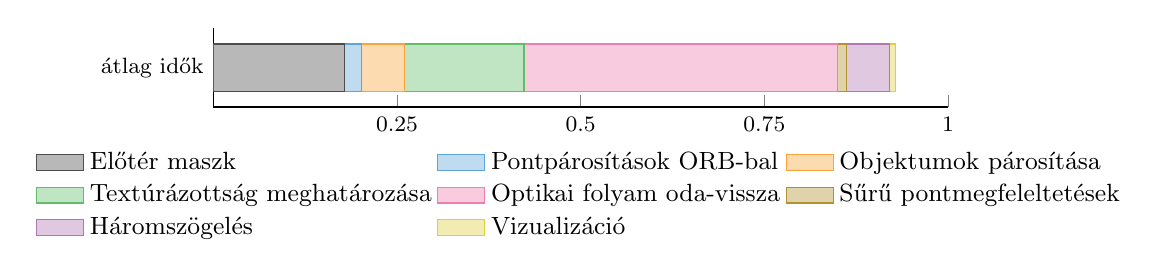
\begin{tikzpicture}
\begin{axis}[
    xbar stacked,
    legend style={
    legend columns=3,
        at={(xticklabel cs:0.5)},
        anchor=north,
        draw=none
    },
    ytick=data,
    axis y line*=none,
    axis x line*=bottom,
    tick label style={font=\footnotesize},
    legend style={font=\footnotesize},
    label style={font=\footnotesize},
    xtick={0.25, 0.5, 0.75, 1},
    width=.9\textwidth,
    bar width=6mm,
    xlabel={Idő másodpercben},
    yticklabels={átlag idők},
    xmin=0,
    xmax=1,
    area legend,
    y=8mm,
    enlarge y limits={abs=0.625},
    legend cell align=left
]
\addplot[color1,fill=color1!40] coordinates {(0.178,0)};
\addplot[color2,fill=color2!40] coordinates {(0.0235,0)};
\addplot[color3,fill=color3!40] coordinates {(0.0583,0)};
\addplot[color4,fill=color4!40] coordinates {(0.163,0)};
\addplot[color5,fill=color5!40] coordinates {(0.427,0)};
\addplot[color6,fill=color6!40] coordinates {(0.0119,0)};
\addplot[color7,fill=color7!40] coordinates {(0.0587,0)};
\addplot[color8,fill=color8!40] coordinates {(0.00845,0)};

\legend{Előtér maszk, Pontpárosítások ORB-bal, Objektumok párosítása, Textúrázottság meghatározása, Optikai folyam oda-vissza, Sűrű pontmegfeleltetések, Háromszögelés, Vizualizáció}
\end{axis}  

\end{tikzpicture}
\caption{Első jelenet esetén az egyes lépések képkockánti átlagos időigénye másodpercben \label{fig:scene1_stats}}
\end{figure}

%----------------------------------------------------------------------------
\section{Párhuzamosítás, többszálúsítás, újra-kalkulált eredmények}
%----------------------------------------------------------------------------

Az előző szekcióbak leírtak alapján látható, hogy szekvenciális végrehajtás mekkora sebességet várhatunk az adott hardveren. A következőkben a párhuzamosításban rejlő lehetőségeket vizsgálom meg.

Különböző platformokon, különböző megoldásokat találhatunk többszálú feladatvégrehajtásra. C++-ban az egyik legelterjedtebb az OpenMP API \cite{OpenMP}. Felhasználásával platform-független, megosztott-memóriás párhuzamos programokat írhatunk. Nagy előnye, hogy ha a cél nem támogatja (legyen az a fordító, vagy a platform), akkor az API megfelelő alkalmazása esetén az alkalmazás ugyanúgy fordítható, azzal a különbséggel, hogy az elkészült bináris csak egy szálon hajtra végje az utasításokat. A következőkben röviden áttekintem az általam használt funkciókat.

A leggyakoribb funkciók deklaratív alapon történnek. 
A legfontosabb koncepció a szál-csoportok. OpenMP esetén az alkalmazás indítása esetén, po




%----------------------------------------------------------------------------
\section{Értékelés}
%----------------------------------------------------------------------------
